\documentclass[11pt, oneside]{article}   	% use "amsart" instead of "article" for AMSLaTeX format
\usepackage{geometry}                		% See geometry.pdf to learn the layout options. There are lots.
\geometry{letterpaper}                   		% ... or a4paper or a5paper or ... 
%\geometry{landscape}                		% Activate for for rotated page geometry
%\usepackage[parfill]{parskip}    		% Activate to begin paragraphs with an empty line rather than an indent
\usepackage{graphicx}				% Use pdf, png, jpg, or eps� with pdflatex; use eps in DVI mode
								% TeX will automatically convert eps --> pdf in pdflatex		
\usepackage{amssymb}
\usepackage{amsmath}
\usepackage{parskip}
\usepackage{color}

\title{Equal areas}
%\author{The Author}
%\section{}
% \subsection*{R code}
\date{}							% Activate to display a given date or no date

\graphicspath{{/Users/telliott_admin/Dropbox/Tex/png/}}

% \begin{center} 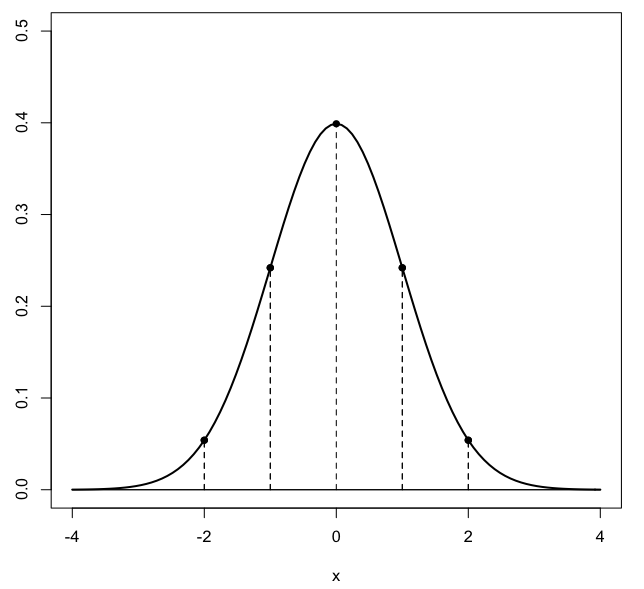
\includegraphics [scale=0.4] {gauss3.png} \end{center}

\begin{document}
\maketitle
\Large
\noindent

Kepler's second law (K2) is the easiest to prove, even without simplifying things by assuming circular orbits.  K2 states that the orbits of the planets (or other satellites) sweep out \emph{equal areas in equal times}.

\subsection*{Newton}

\begin{center} 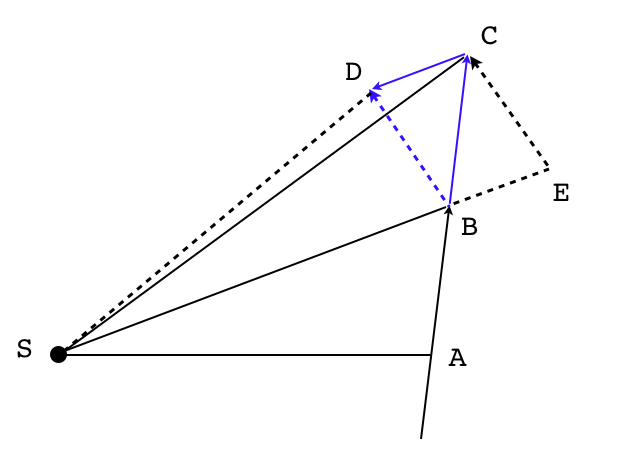
\includegraphics [scale=0.5] {newton_area.png} \end{center}

We diagram the sun $S$ and a planet at $A$.  Imagine that the force toward the sun is applied discretely.  That is, for a sufficiently small interval, the planet travels from $A$ to $B$ at constant velocity and if undisturbed, would travel to $C$ in the next unit of time.  

Because there is no force, the velocity is constant and so the length of $AB$ is the same as that of $BC$, and since $AB$ is on the same line as $BC$, the area of $\triangle ABS$ is equal to the area of $\triangle BCS$.  

(Draw the vertical line from $S$ to the line containing $ABC$.  The area is one-half the length of that altitude times the distance, either $AB$ or $BC$).

Now, suppose the force is applied at $B$ toward the sun along $EBS$.  As a result, the trajectory $BC$ is modified by addition of a new component (the velocity from the force times unit time).  Call that component $CD$ and add it to $BC$ to give the actual trajectory, $BD$.  

Note that $CD$ is parallel to $SBE$, it is the change in velocity resulting from application of the force toward the sun.  Because of that, any point on $CD$ can be used to draw a triangle with the same base $SB$ and the result will have the equal area no matter which point is chosen.

In particular, the area of $\triangle BDS$ is equal to the area of $\triangle BCS$, which was found earlier to be equal to the area of $\triangle ABS$.  Since the two triangles from the actual motion have the same area, the area is constant.

\subsection*{Feynman}

Richard Feynman gave a famous series of talks at Cornell in 1964 that were videotaped.  Bill Gates later purchased them and put them on the web, unfortunately with some Microsoft DRM.  Still, I have the book, called \emph{The Character of Physical Law}.  The argument I use here is from Chapter 2, \emph{The Relation of Mathematics to Physics}.

It depends on a tiny bit of calculus (specifically, the product rule for differentiation).  It also uses the fact that the product rule is valid for vector cross products.  (See the short write-up on cross-products for a proof).

The basic idea is that if we have two vectors $\mathbf{a}$ and $\mathbf{b}$ which are functions of time, then

\[ \frac{d}{dt} \ (\mathbf{a} \times \mathbf{b}) = \frac{d\mathbf{a}}{dt} \times \mathbf{b} + \mathbf{a}  \times \frac{d\mathbf{b}}{dt}    \]

In our application the two vectors are the position vector of the planet with respect to the sun, $\mathbf{r}$, and the time-derivative of that vector.

\[ \frac{d\mathbf{r}}{dt} = \mathbf{v} \]

Or, as the physicists would write it, using Newton's dot notation for the time-derivative:

\[ \mathbf{v} = \dot{\mathbf{r}} \]

We are interested in the area of the triangle formed by the vectors $\mathbf{r}$ and $\dot{\mathbf{r}}$ over a small interval of time, $dt$.  A nice feature of the vector cross-product is that it provides this area (actually twice the area).  Namely

\[ A =  \mathbf{a} \times \mathbf{b} = |\mathbf{a}| |\mathbf{b}| \sin \theta   \]

where $\theta$ is the angle between $\mathbf{a}$ and $\mathbf{b}$, and A is the area.

Our hypothesis is that the area $A$ is the same no matter where the planet is in its orbit.  Another way to say the same thing is that A doesn't change with time

\[ \dot A = 0 \]

Now 

\[ A = \mathbf{r} \times \dot{\mathbf{r}} \]

and I hope you can see why we want to compute $\dot A$.  Using the product rule that we had above it's easy.  Namely

\[ \dot A = \frac{d}{dt} \ (\mathbf{r} \times \dot{\mathbf{r}}) \]
\[ \dot A = \dot{\mathbf{r}} \times \dot{\mathbf{r}} \ + \ \mathbf{r} \times \ddot{\mathbf{r}} \]

As Feynman says: it's just playing with dots.

So let's look at those two terms.  Another nice fact about the cross-product is that if the two vectors point in the same direction, then the cross-product is zero.

Any vector points in the same direction as itself, so the first term is certainly zero.  

\[ \dot{\mathbf{r}} \times \dot{\mathbf{r}} \ = 0 \]

Next, recall that the second derivative with respect to time of the position is the acceleration vector.  According to Newton's second law, the force of gravity points toward the sun, radially.  

But of course the position vector also points out radially from the sun.  $\mathbf{r}$ and $\ddot{\mathbf{r}}$ are in the same direction (the opposite direction \emph{is} the same direction, multiplied by $-1$), so the cross-product is again zero.

\[ \mathbf{r} \times \ddot{\mathbf{r}} \ = 0 \]

So that means the whole thing is zero.

\[ \dot A = \dot{\mathbf{r}} \times \dot{\mathbf{r}} \ + \ \mathbf{r} \times \ddot{\mathbf{r}} = 0 + 0 = 0  \]

We have shown that the area is constant.

\end{document}  